\PassOptionsToPackage{dvipsnames,svgnames,table}{xcolor}
\documentclass[11pt]{article}
\usepackage[a4paper,margin=22mm]{geometry}
\usepackage[no-math]{fontspec}
\setmainfont{DejaVu Serif}
\usepackage{amsmath,amssymb,amsthm,mathtools,graphicx,xcolor,hyperref,xurl,xspace,ifthen,enumerate}
\usepackage[shortlabels]{enumitem}
\setlength{\emergencystretch}{4em}
\AtBeginDocument{\special{pdf:mapline pzdr Dingbats <uzdr.pfb}}
\SetMathAlphabet{\mathbf}{normal}{OT1}{cmr}{bx}{n}
\SetMathAlphabet{\mathbf}{bold}{OT1}{cmr}{bx}{n}
\newtheorem{theo}{Theorem}[section]
\newtheorem{lemm}[theo]{Lemma}
\newtheorem{thm}[theo]{Theorem}
\newtheorem{proposition}[theo]{Proposition}
\newtheorem{corollary}[theo]{Corollary}
\newtheorem{definition}[theo]{Definition}
\newtheorem{theorem}[theo]{Theorem}
\newtheorem*{remas*}{Remarks}
\newtheorem{remas}[theo]{Remarks}
\newtheorem*{exam*}{Example}
\newtheorem{ques}[theo]{Question}
\providecommand{\og}{«\nobreakspace}
\providecommand{\fg}{\nobreakspace»}
\newtheorem{lem}[theo]{Lemma}
\newtheorem{lemma}[theo]{Lemma}
\newtheorem{prop}[theo]{Proposition}
\newtheorem{coro}[theo]{Corollary}
\newtheorem{corol}[theo]{Corollary}
\newtheorem*{conj*}{Conjecture}
\newtheorem{conj}[theo]{Conjecture}
\newtheorem{conjecture}[theo]{Conjecture}
\newtheorem{Proposition}[theo]{Proposition}
\newtheorem{theoreme}[theo]{Theorem}
\theoremstyle{definition}
\newtheorem{defi}[theo]{Definition}
\newtheorem{exam}[theo]{Example}
\newtheorem{exem}[theo]{Example}
\newtheorem{remark}[theo]{Remark}
\newtheorem{example}[theo]{Example}
\newtheorem{rema}[theo]{Remark}
\newtheorem{nota}[theo]{Notation}
\newtheorem{notation}[theo]{Notation}
\newtheorem*{notas}{Notations}
\newtheorem{result}[theo]{Result}
\newtheorem{question}[theo]{Question}
\newtheorem{prob}[theo]{Problem}
\newtheorem*{rema*}{Remark}
\newtheorem*{defi*}{Definition}
\newtheorem*{theo*}{Theorem}
\newtheorem*{lemm*}{Lemma}
\newtheorem*{prop*}{Proposition}
\newcommand{\enoncename}{}
\newtheorem{corpusenonce}[theo]{\enoncename}
\newenvironment{enonce}[2][]{\renewcommand{\enoncename}{#2}\begin{corpusenonce}}{\end{corpusenonce}}
\newenvironment{enonce*}[2][]{\par\medskip\noindent\textbf{#2.}\itshape}{\par\medskip}
\newenvironment{proofc}[1][\proofname]{\begin{proof}[#1]}{\end{proof}}
\newcommand{\Mc}{\mathcal{M}}
\newcommand{\pointir}{.\ ---\ }
\newcommand{\equalenv}[2]{\expandafter\let\csname#1\expandafter\endcsname\csname#2\endcsname\expandafter\let\csname end#1\expandafter\endcsname\csname end#2\endcsname}
\providecommand{\diagbox}[3][]{\begin{tikzpicture}[x=1em,y=1em,baseline=(current bounding box.center)]\useasboundingbox(0,0) rectangle(3,1.4);\draw(0,1.4)--(3,0);\node at(.5,.3){#2};\node at(2.5,1.1){#3};\end{tikzpicture}}
\providecommand{\eg}{e.g.\ }
\providecommand{\ie}{i.e.\ }
\providecommand{\cf}{cf.\ }

\providecommand{\mathof}[1]{\mathrm{#1}}

\numberwithin{equation}{section}


\def\endappendix{}


\usepackage{tikz}
\usetikzlibrary{arrows,decorations.pathreplacing,calc}

\newcommand{\RR}{\mathbb{R}}
\newcommand{\ZZ}{\mathbb{Z}}
\DeclareMathOperator{\codim}{codim}
\DeclareMathOperator{\Conv}{Conv}
\DeclareMathOperator{\MV}{MV}
\DeclareMathOperator{\Span}{Span}
\DeclareMathOperator{\trop}{trop}
\DeclareMathOperator{\val}{val}

\makeatletter
\newtheorem*{rep@theorem}{\rep@title}
\newcommand{\newreptheorem}[2]{
\newenvironment{rep#1}[1]{
 \def\rep@title{#2 \ref{##1}}
 \begin{rep@theorem}}
 {\end{rep@theorem}}}
\makeatother
\newreptheorem{theorem}{Theorem}


















\begin{document}
\section*{\raggedright 827: Every component of tropical hypersurface intersections meets a nonempty stable intersection}
\noindent\textbf{Author:} Ren, Yue\par\noindent\textbf{Source:} On intersections and stable intersections of tropical hypersurfaces. Algebraic Combinatorics 7 (2024), publisher version, DOI 10.5802/alco.327. \url{https://alco.centre-mersenne.org/articles/10.5802/alco.327/}
\par\noindent\textbf{License:} CC BY 4.0, \url{https://creativecommons.org/licenses/by/4.0/}. The original publisher PDF cover has the explicit license notice. See the saved source/license records.
\par\noindent\textbf{Editorial material note (not author text):} The selected problem is Theorem3.3 with the exact tropical-hypersurface and nonempty-stable-intersection hypotheses. Full native Sections1--3 retain affine-subspace intersection control, generic-coefficient irreducibility/Zariski-dense translation component argument, and complete maximal-subfamily proof, together with all original native TikZ figures. Yu generic prime ideal and named tropical structure/stable tropicalization results remain explicit standard prerequisites. Later open questions are unselected; no general balanced-polyhedral extension or empty-stable-intersection conclusion is claimed. All proof text and formulas below are editable author TeX. Mathematical wording, language and proof order are retained. Only the article class, title matter and bibliography presentation are adapted for independent compilation; no proof has been generated or repaired.
\par\noindent\textbf{Editorial difficulty:} H2: The proof first establishes uniform stable-intersection emptiness across components by separating support-degenerate and irreducible generic-coefficient cases. A Zariski-density translation argument supplies the key component control; a maximal-subfamily argument then forces stable-intersection points in each ordinary component. This is not a formal dimension or balancing check.
\medskip\hrule\medskip
\noindent\textbf{Author statement, complete proof and local supporting text follow in source order.}
\section{Introduction}

Tropical varieties are commonly described as combinatorial shadows of algebraic varieties. The tropicalization of an algebraic variety shares many common properties with its algebraic counterpart, such as its dimension \cite[Structure Theorem 3.3.5]{MaclaganSturmfels15}. This has prominently been used to show finiteness of central configurations in four and five body problems of celestial mechanics \cite{HamptonMoeckel06,HamptonJensen11}, as well as central configurations with restrictions on their geometry rather than the number of bodies~\cite{HamptonJensen15,DengHampton23}. In these proofs, the authors rely on the fact that their central configurations satisfy certain algebraic equations and thus lie on an algebraic variety. They then show that the tropicalization of the algebraic variety is zero-dimensional by intersecting tropical hypersurfaces and eliminating all resulting positive-dimensional polyhedra. Intersections of tropical hypersurfaces are also used in the study of Lagrangian rational homology spheres in Calabi-Yau threefolds \cite{MakRuddat20}.

Computing an intersection of tropical hypersurfaces can however be an incredibly challenging task. Tropical hypersurfaces may have many maximal polyhedra and the computation requires intersecting all combinations thereof. While parallelisation and a clever choice of intersection order can lead to significant improvements in performance \cite{JSV17}, there is no definite way to avoid the exponential blowup in the number of intersections required. This circumstance is especially unsatisfying when one expects the final intersection to be very small, such as in the aforementioned applications.

One alternative would be to compute the intersection ``bottom-up'': if one can identify at least one point in every connected component of the intersection, then the remaining points can be obtained using a traversal as in the computation of tropical varieties \cite{BJST07,MR20}. When the number of hypersurfaces does not exceed the ambient dimension, a natural candidate for such a set of starting points is their stable intersection. The stable intersection can be computed quickly using techniques such as tropical homotopy continuation \cite{Jensen16}. And, due to the similarity in their definitions, it is not unreasonable to expect every connected component of the intersection to contain a point of the stable intersection, see Figure~\ref{fig:stableIntersection}. However, until now there has been no known proof of that statement. This paper aims to close that gap:

\begin{reptheorem}{thm:main}
  Let $\Sigma_1,\dots\Sigma_k$ be tropical hypersurfaces in $\RR^n$ with a non-empty stable intersection $\bigwedge_{i=1}^k\Sigma_i\neq\emptyset$. Then, every connected component of their intersection $\bigcap_{i=1}^k|\Sigma_i|$ contains a point in the support of their stable intersection $|\bigwedge_{i=1}^k\Sigma_i|$.
\end{reptheorem}

Despite the obvious combinatorial nature of the statement, our proof relies on an algebro-geometric result by Josephine Yu on generic polynomials generating prime ideals \cite{Yu16}, and the structural properties of tropicalizations of irreducible varieties.

\begin{figure}
  \centering

  \begin{tikzpicture}
    \node at (-3.5,0)
    {
      \begin{tikzpicture}[scale=0.9]
        \draw[blue!50!black,very thick]
        (-1,2) -- ++(1,1)
        (-1,2) -- ++(-2,0)
        (-1,2) -- (-1,1)
        (-1,1) -- ++(-2,0)
        (-1,1) -- (0,0)
        (0,0) -- ++(0,-1)
        (0,0) -- (1,0)
        (1,0) -- ++(0,-1)
        (1,0) -- ++(1.5,1.5);

        \draw[red!70!black,very thick]
        (0.85,-0.5) -- ++(-3.5,3.5)
        (0.85,-0.5) -- ++(0,-0.5)
        (0.85,-0.5) -- ++(1.65,1.65);

        \draw[fill=white]
        (-1.65,2) circle (2pt)
        (-1,1.35) circle (2pt)
        (0.35,0) circle (2pt)
        (1,-0.35) circle (2pt);

        \draw[->,densely dotted,very thick,violet]
        (0.5,-0.65) -- node[below,font=\footnotesize,xshift=-0.5mm] {$v$} (0.85,-0.65);
      \end{tikzpicture}
    };
    \draw[->,very thick,violet] (-0.8,-1) -- node[below] {$v\rightarrow 0$} (0.8,-1);
    \node at (3.5,0)
    {
      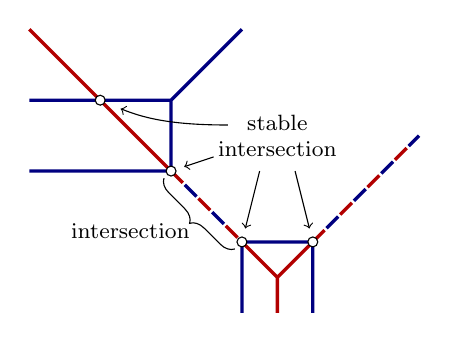
\begin{tikzpicture}[scale=0.9]
        \draw[blue!50!black,very thick]
        (-1,2) -- ++(1,1)
        (-1,2) -- ++(-2,0)
        (-1,2) -- (-1,1)
        (-1,1) -- ++(-2,0)
        (0,0) -- ++(0,-1)
        (0,0) -- (1,0)
        (1,0) -- ++(0,-1);

        \draw[red!70!black,very thick]
        (-1,1) -- ++(-2,2)
        (0,0) -- (0.5,-0.5)
        (0.5,-0.5) -- ++(0,-0.5)
        (0.5,-0.5) -- (1,0);

        \draw[blue!50!black,very thick,dash pattern= on 6pt off 8pt,dash phase=7pt]
        (-1,1) -- (0,0)
        (1,0) -- ++(1.5,1.5);
        \draw[red!70!black,very thick,dash pattern= on 6pt off 8pt]
        (-1,1) -- (0,0)
        (1,0) -- ++(1.5,1.5);

        \draw[fill=white]
        (-2,2) circle (2pt)
        (-1,1) circle (2pt)
        (0,0) circle (2pt)
        (1,0) circle (2pt);
        \draw[decorate,decoration={brace,amplitude=5pt,mirror}] ($(-1,1)+(-0.1,-0.1)$) -- node[font=\footnotesize,anchor=north east] {intersection} ($(0,0)+(-0.1,-0.1)$);
        \node[font=\footnotesize,text width=20mm,align=center] at (0.5,1.5) {stable\\ intersection};
        \draw[<-,shorten <=5pt] (0,0) -- ++(0.25,1);
        \draw[<-,shorten <=5pt] (1,0) -- ++(-0.25,1);
        \draw[<-,shorten <=5pt] (-1,1) -- ++(0.6,0.2);
        \draw[<-,shorten <=8pt] (-2,2) to[out=337.5,in=180] ++(1.8,-0.35);
      \end{tikzpicture}
    };
  \end{tikzpicture}\vspace{-3mm}
  \caption{The intersection and stable intersection of two tropical plane curves. Notice how every connected component of the intersection contains a point in the stable intersection.}
  \label{fig:stableIntersection}
\end{figure}

\section{Background}

In this article, we closely follow the notation of \cite{MaclaganSturmfels15}. In particular:

\begin{notas}
  For the remainder of the paper, we will fix an algebraically closed field $K$ of characteristic $0$ with non-trivial valuation $\val\colon K^\ast\rightarrow\RR$.
  Let $K[x^{\pm1}]\coloneqq K[x_1^{\pm1},\dots,x_n^{\pm1}]$ be a multivariate (Laurent) polynomial ring thereover.
\end{notas}

For the sake of brevity, we will abbreviate ``pure, weighted, balanced polyhedral complex'' by ``balanced polyhedral complex'', and we will consider tropical hypersurfaces as balanced polyhedral complexes instead of supports thereof. Additionally, we will denote the stable intersection by ``$\wedge$'' for better inline formatting.

We will further assume some familiarity with the basic concepts in Sections 2 and~3 of \cite{MaclaganSturmfels15}, such as the duality between tropical hypersurfaces and regular subdivisions of Newton polytopes, tropicalizations of algebraic varieties, stable intersections of balanced polyhedral complexes, and mixed volumes of polytopes. In particular, we will be using the following results:

\begin{theorem}[{\cite[Theorem 3.3.5]{MaclaganSturmfels15}} Structure Theorem for Tropical Varieties]\label{thm:StructureTheorem}
  Let $X$ be an irreducible variety in $(K^\ast)^n$ of dimension $d$. Then, $\trop(X)$ is the support of a balanced polyhedral complex in $\RR^n$ of dimension $d$ that is connected in codimension $1$.
\end{theorem}

\begin{theorem}[{\cite[Theorem 3.6.1]{MaclaganSturmfels15}}]\label{thm:stableTropicalization}
  Let $\Sigma_1,\Sigma_2$ be two balanced polyhedral complexes in $\RR^n$ whose support is the tropicalization of two varieties $X_1,X_2\subseteq (K^\ast)^n$. Then, there is a Zariski dense subset $U\subseteq (K^\ast)^n$ consisting of elements with component-wise valuation $0$ such that
  \[ |\Sigma_1\wedge\Sigma_2| = \trop(X_1\cap z\cdot X_2) \qquad \text{for all }z\in U. \]
\end{theorem}

\begin{theorem}[{\cite[Theorem 3.6.10]{MaclaganSturmfels15}}]\label{thm:stableIntersection}
  Let $\Sigma_1,\Sigma_2$ be two balanced polyhedral complexes in $\RR^n$ of codimension $d$ and $e$, respectively. If the stable intersection $\Sigma_1\wedge\Sigma_2$ is non-empty, then it is a balanced polyhedral complex of codimension $d+e$.
\end{theorem}

Additionally, we will require the following theorem by Yu. Whilst {\cite[Theorem~3]{Yu16}} is more general and also covers fields of positive characteristic, we will only need and state its specialisation to fields of characteristic $0$. In the theorem, ``general polynomials'' means polynomials whose coefficients lie in a fixed Zariski open, dense set of the coefficient space.

\begin{theorem}[{\cite[Theorem 3]{Yu16}}]\label{thm:Yu}
  Let $A_1,\dots,A_k\subseteq\ZZ^n$, $k\leq n$, and $0\in A_i$ for all $i=1,\dots,k$. General polynomials in $K[x]$ with monomial supports $A_1,\dots,A_k$ generate a proper ideal whose radical is prime if and only if for every $\emptyset\neq J\subseteq [k]$ one of the following holds:
  \begin{enumerate}
  \item\label{enumitem:Yu1} $\dim \Span\bigcup_{j\in J}A_j>|J|$, or
  \item\label{enumitem:Yu2} $\dim \Span\bigcup_{j\in J}A_j=|J|$ and $\MV(\Conv(A_j)\mid j\in J)=1$.
  \end{enumerate}
\end{theorem}

\section{Main Theorem}

In this section, we prove Theorem~\ref{thm:main}, beginning with two lemmas. In the first lemma, we regard affine subspaces as balanced polyhedral complexes consisting of a single polyhedron. We show that if an affine subspace has an empty stable intersection with a balanced polyhedral complex, then so do its translates, see Figure~\ref{fig:subspaceIntersection}.

\begin{figure}
  \centering
  \begin{tikzpicture}
    \node at (0,0)
    {
      \begin{tikzpicture}[x={(90:4mm)},y={(0:4mm)},z={(240:4mm)}]
        \draw[very thick]
        (0,0,0)++(0,-1.5,1.5) -- ++(0,-1.5,1.5)
        (0,0,0)++(0,-1.5,-1.5) -- ++(0,-1.5,-1.5)
        (0,0,0) -- (0,2.5,0)
        (0,5,0) -- ++(0,1.5,1.5)
        (0,5,0) -- ++(0,1.5,-1.5);
        \fill[blue!20,opacity=0.6] (-1.5,-1.5,-3) -- (-1.5,-1.5,3) -- (1.5,-1.5,3) -- (1.5,-1.5,-3) -- cycle;
        \fill[blue!20,opacity=0.6] (-1.5,2.5,-3) -- (-1.5,2.5,3) -- (1.5,2.5,3) -- (1.5,2.5,-3) -- cycle;
        \fill[blue!20,opacity=0.6] (-1.5,6.5,-3) -- (-1.5,6.5,3) -- (1.5,6.5,3) -- (1.5,6.5,-3) -- cycle;
        \draw[very thick] (0,2.5,0) -- (0,5,0)
        (0,0,0) -- ++(0,-1.5,1.5)
        (0,0,0) -- ++(0,-1.5,-1.5)
        (0,5,0)++(0,1.5,1.5) -- ++(0,1.5,1.5)
        (0,5,0)++(0,1.5,-1.5) -- ++(0,1.5,-1.5);
        \fill[blue!70!black] (0,-1.5,1.5) circle (2pt)
        (0,-1.5,-1.5) circle (2pt)
        (0,2.5,0) circle (2pt)
        (0,6.5,1.5) circle (2pt)
        (0,6.5,-1.5) circle (2pt);
        \fill
        (0,0,0) circle (2pt)
        (0,5,0) circle (2pt);
        \node[anchor=north west,blue!70!black] at (-1.5,-1.5,3) {$L'$};
        \node[anchor=north west,blue!70!black] at (-1.5,2.5,3) {$L$};
        \node[anchor=north west,blue!70!black] at (-1.5,6.5,3) {$L''$};
        \node[anchor=south] at (0,0.85,0) {$\Sigma$};
      \end{tikzpicture}
    };
    \node at (6,0)
    {
      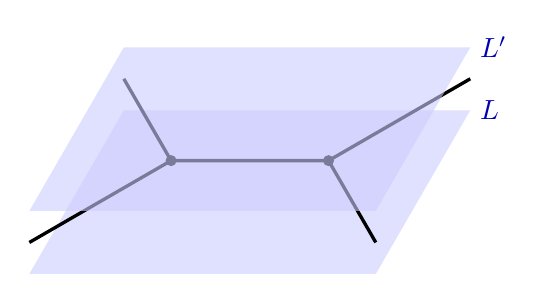
\begin{tikzpicture}[x={(90:4mm)},y={(0:4mm)},z={(240:4mm)}]
        \fill[blue!20,opacity=0.6] (-1,-3,-3) -- (-1,-3,3) -- (-1,8,3) -- (-1,8,-3) -- cycle;
        \draw[very thick]
        (0,0,0) -- ++(0,-3,3)
        (0,0,0) -- ++(0,-3,-3)
        (0,0,0) -- (0,2.5,0)
        (0,5,0) -- ++(0,3,3)
        (0,5,0) -- ++(0,3,-3)
        (0,2.5,0) -- (0,5,0);
        \fill
        (0,0,0) circle (2pt)
        (0,5,0) circle (2pt);
        \fill[blue!20,opacity=0.6] (1,-3,-3) -- (1,-3,3) -- (1,8,3) -- (1,8,-3) -- cycle;
        \node[anchor=west,blue!70!black] at (-1,8,-3) {$L$};
        \node[anchor=west,blue!70!black] at (1,8,-3) {$L'$};
      \end{tikzpicture}
    };
  \end{tikzpicture}\vspace{-3mm}
  \caption{A fixed balanced polyhedral complex $\Sigma$ with different translates of an affine subspace.  Notice how the stable intersection is either always non-empty (left) or empty (right), but not both.}
  \label{fig:subspaceIntersection}
\end{figure}

\begin{lemma}\label{lem:subspaceIntersection}
  Let $\Sigma$ be a balanced polyhedral complex in $\RR^n$. Let $L, L'$ be two parallel affine subspaces in $\RR^n$, i.e., $L=\mathrm{Ker}(A)+v$ and $L'=\mathrm{Ker}(A)+v'$ for some matrix $A\in\RR^{k\times n}$ and vectors $v,v'\in\RR^n$. Then
  \[ L\wedge\Sigma=\emptyset\quad\Longleftrightarrow\quad L'\wedge\Sigma=\emptyset. \]
\end{lemma}
\begin{proof}
  Without loss of generality, we may assume that $L$ is a linear space, i.e., $0\in L$. Note that both $L$ and $L'$ are supports of stable intersections of affine hyperplanes, i.e., $L=|H_1\wedge\dots\wedge H_k|$ and $L'=|(H_1+v')\wedge H_2\wedge\dots\wedge H_k|$ for suitable hyperplanes $H_1,\dots,H_k$ and $v'\in\RR^n$. Since $H_1$ and $H_1+v'$ remain parallel affine subspaces, and $H_2\wedge\dots\wedge H_k\wedge\Sigma$ remains a balanced polyhedral complex by Theorem~\ref{thm:stableIntersection}, we may assume without loss of generality that $L$ is a hyperplane and $L'$ is an affine hyperplane.

  Consider the projection of $|\Sigma|$ to the one-dimensional orthogonal complement~$L^\perp$. The image of the projection remains the support of a balanced polyhedral complex, which means it is either finite or the entire complement.
  If the projection is finite, then $\Sigma$ is contained in a union of affine hyperplanes parallel to $L$ and $L'$, and we have $L\wedge\Sigma=\emptyset=L'\wedge\Sigma$. If the projection is the entire complement, then we have  $L\wedge\Sigma\neq\emptyset\neq L'\wedge\Sigma$.
\end{proof}

In the next lemma, the connected component of a balanced polyhedral complex $\Sigma$ is a maximal polyhedral subset  $\Gamma\subseteq\Sigma$ such that $|\Gamma|$ is a connected component of $|\Sigma|$.  Note that $\Gamma$ is naturally a balanced polyhedral complex.  We use Lemma~\ref{lem:subspaceIntersection} to prove a similar statement but for connected components of a stable intersection of tropical hypersurfaces instead of translates of an affine subspace.

\begin{lemma}\label{lem:stableConspiracy}
  Let $\Sigma_1,\dots,\Sigma_k,\Sigma_{k+1}$ be tropical hypersurfaces in $\RR^n$ with $\bigwedge_{i=1}^k\Sigma_i\neq\emptyset$. Then for any two connected components $\Gamma,\Gamma'\subseteq \bigwedge_{i=1}^k\Sigma_i$ we have
  \[ \Gamma\wedge\Sigma_{k+1}=\emptyset \quad\Longleftrightarrow\quad \Gamma'\wedge\Sigma_{k+1}=\emptyset. \]
\end{lemma}
\begin{proof}
  Let $A_1,\dots,A_k\subseteq\ZZ^n$ be monomial supports of polynomials with tropical hypersurfaces $\Sigma_1,\dots,\Sigma_k$ and $0\in A_i$ for all $i$. We distinguish between two cases:
  \begin{description}[leftmargin=0 pt]
  \item[Case 1] If $A_1,\dots,A_k$ do not satisfy Conditions \eqref{enumitem:Yu1} or \eqref{enumitem:Yu2} of Theorem~\ref{thm:Yu}, then there is a subset $J\subseteq [k]$ such that $\dim \Span (\bigcup_{j\in J} A_j)\leq |J|$.
    Note that the lineality space of $\bigwedge_{j\in J}\Sigma_j$ contains the orthogonal complement of $\Span (\bigcup_{j\in J} A_j)$. Therefore, the lineality space of $\bigwedge_{j\in J}\Sigma_j$ has codimension at most $|J|$. And since $\bigwedge_{j\in J}\Sigma_j\supseteq\bigwedge_{i=1}^k\Sigma_i \neq\emptyset$, Theorem~\ref{thm:stableIntersection} implies that $\bigwedge_{j\in J}\Sigma_j$ has codimension exactly $|J|$. Hence,~$|\bigwedge_{j\in J}\Sigma_j|=L_1\cup \dots\cup L_r$, where $L_1,\dots,L_r$ are affine subspaces parallel to its lineality space. The claim follows by applying Lemma~\ref{lem:subspaceIntersection} to $\Sigma\coloneqq\bigwedge_{i\in [k+1]\setminus J}\Sigma_i$ and the affine subspaces~$L_1,\dots,L_r$.
  \item[Case 2] If $A_1,\dots,A_k$ satisfy Conditions \eqref{enumitem:Yu1} or \eqref{enumitem:Yu2} of Theorem~\ref{thm:Yu}, consider
  \begin{itemize}
  \item $K\cdot x^A\coloneqq \bigoplus_{i=1}^k \bigoplus_{\alpha\in A_i} K\cdot x^{\alpha}$, the vector space of polynomial tuples $(f_1,\dots,f_k)$ where $f_i$ has monomial support $A_i$, and
  \item $K^{|A|}\coloneqq K^{|A_1|+\dots+|A_k|}$, their coefficient space.
  \end{itemize}
  In particular, any choice of coefficients $c=(c_{i,\alpha})_{i\in [k], \alpha\in A_i}\in K^{|A|}$ defines a tuple of polynomials $f(c)\coloneqq (f_i(c))_{i\in [k]}\in K\cdot x^A$ with $f_i(c)\coloneqq\sum_{\alpha\in A_i}c_{i,\alpha}x^\alpha$ and vice versa. By Theorem~\ref{thm:Yu}, there is a Zariski open, dense subset $U\subseteq K^{|A|}$ such that any $c\in U$ yields an $f(c)$ whose entries generate an ideal whose radical is prime. By Theorem~\ref{thm:StructureTheorem}, the tropicalization $\trop(V(f(c)))\coloneqq \trop(V(\langle f_1(c),\dots,f_k(c)\rangle))$ will be connected for any $c\in U$. We will now show that there is a $c_0\in U$ for which $\trop(V(f(c_0)))=|\bigwedge_{i=1}^k\Sigma_i|$, so that the claim holds trivially as there is only one connected component.

  Pick any $c\in U$. By Theorem~\ref{thm:stableTropicalization}, combined with a simple induction on $k$, there is a Zariski dense $S\subseteq ((K^\ast)^n)^{k-1}$ with $\trop(V(f_1(c))\cap z_2V(f_2(c))\cap\cdots\cap z_kV(f_k(c)))=|\bigwedge_{i=1}^k\Sigma_i|$ for all ${(z_2,\dots,z_k)\in S}$. Then for any $z=(z_2,\dots,z_k)\in ((K^\ast)^n)^{k-1}$, let $z^{-1}\cdot c\in K^{|A|}$ denote the coefficients of the polynomials $f_1(z^{-1}\cdot c)=\sum_{\alpha\in A_1}c_{1,\alpha} x^\alpha$ and $f_i(z^{-1}\cdot c)=\sum_{\alpha\in A_i}c_{i,\alpha} z_i^{-\alpha}x^\alpha$ for $i>1$, so that $V(f_1(z^{-1}c))=V(f_1(c))$ and $V(f_i(z^{-1}c))=z_i V(f_i(c))$ for $i>1$. Consider the rational map
  \[ \varphi\colon\quad ((K^\ast)^n)^{k-1}\rightarrow K^{|A|}, \qquad z\mapsto z^{-1}\cdot c. \]
  The preimage $\varphi^{-1}(U)$ is a Zariski open set, and, since $\varphi(1,\dots,1)=c\in U$, $\varphi^{-1}(U)$ is non-empty. Thus $\varphi^{-1}(U)$ has to intersect the Zariski dense set $S$, and any point in the image of the intersection gives us the desired $c_0\in U$. \qedhere
  \end{description}
\end{proof}

Using Lemma~\ref{lem:stableConspiracy} we can now prove:

\pgfdeclareverticalshading{howTheHellDoesThisWork}{4cm}{color(0cm)=(white);color(2.95cm)=(white);color(3.25cm)=(blue!20);color(6cm)=(white)}
\begin{figure}[t]
  \centering
  \begin{tikzpicture}
    \node (left)
    {
      \begin{tikzpicture}[x={(240:9mm)},y={(0:9mm)},z={(90:9mm)},shading angle from/.style args={line from #1 to #2}{insert path={let \p1=($#2-#1$),\n1={atan2(\y1,\x1)} in},shading angle=\n1}]
        \fill[shading=howTheHellDoesThisWork, shading angle from={line from (-1.5,0,0) to (1.5,0,0)}]  (-2.625,-0.75,0) -- (-1.5,0,0) -- (1.5,0,0) -- (2.625,-0.75,0) -- cycle;
        \draw[very thick, white] (2.625,-0.75,0) -- (-2.625,-0.75,0);
        \draw[thick, blue!40!black] (-3,-1,0) -- (-1.5,0,0) -- (1.5,0,0) -- (3,-1,0);
        \node[anchor=north east, blue!40!black] at (-3,-1,0) {$C$};

        \draw[red!70!black,thick]
        (0,1,0) -- node[above] {$\gamma$} (0,2.25,0)
        (0,0,0) -- (0,-1,0)
        (0,-1,0) -- (1,-2,0)
        (0,-1,0) -- (-1,-2,0)
        (1,-2,0) -- (2,-2,0)
        (1,-2,0) -- (1,-3,0)
        (-1,-2,0) -- node[above] {$\Gamma$} (-1,-3,0)
        (-1,-2,0) -- (-2,-2,0);

        \draw[violet!70!black,->,very thick] (0,0,0) -- (0,1,0);
        \fill[violet!70!black] (0,0,0) circle (3pt);
        \node[anchor=north west,violet!70!black,xshift=-1mm,yshift=-2mm] at (0,0,0) {$w$};
        \node[anchor=north,violet!70!black,xshift=-1mm,yshift=-2mm] at (0,1,0) {$u$};
      \end{tikzpicture}
    };
    \node (right) at (6.5,0)
    {
      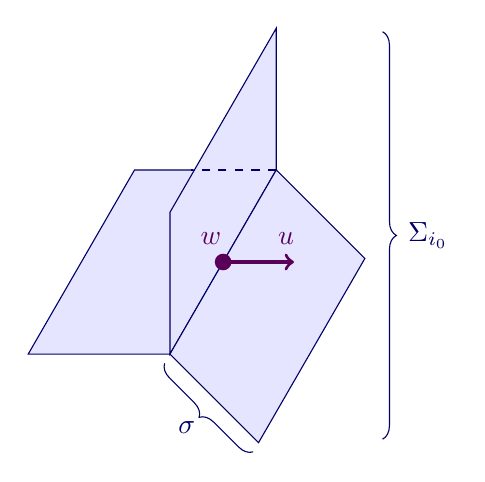
\begin{tikzpicture}[x={(240:9mm)},y={(0:9mm)},z={(90:9mm)}]
        \phantom
        {
          \draw[thick, blue!40!black] (-3,-1,0) -- (-1.5,0,0) -- (1.5,0,0) -- (3,-1,0);
        }
        \draw[blue!40!black,fill=blue!10] (-1.5,-2,0) -- (-1.5,0,0) -- (1.5,0,0) -- (1.5,-2,0) -- cycle;
        \draw[blue!40!black,fill=blue!10] (-1.5,0,2) -- (-1.5,0,0) -- (1.5,0,0) -- (1.5,0,2) -- cycle;
        \draw[blue!40!black,dashed] (-1.5,0,0) -- ++(0,-1.2,0);
        \draw[blue!40!black,fill=blue!10] (-1.5,1.25,-1.25) -- (-1.5,0,0) -- (1.5,0,0) -- (1.5,1.25,-1.25) -- cycle;

        \draw[violet!70!black,->,very thick] (0,0,0) -- (0,1,0);
        \fill[violet!70!black] (0,0,0) circle (3pt);
        \node[anchor=south east,violet!70!black,xshift=1mm,yshift=1mm] at (0,0,0) {$w$};
        \node[anchor=south,violet!70!black,xshift=-1mm,yshift=1mm] at (0,1,0) {$u$};
        \draw[blue!40!black,decorate,decoration={brace,amplitude=5pt,mirror}] (0,2.25,-2.5) -- node[anchor=west,xshift=2mm] {$\Sigma_{i_0}$} (0,2.25,3.25);
        \draw[blue!40!black,decorate,decoration={brace,amplitude=5pt,mirror}] (1.65,0,0) -- node[anchor=north east,xshift=-0.5mm,yshift=-0.5mm] {$\sigma$} (1.65,1.25,-1.25);
      \end{tikzpicture}
    };
  \end{tikzpicture}\vspace{-2mm}
  \caption{Illustrations for the proof of Theorem~\ref{thm:main}. $C$ is a connected component of $\bigcap_{i=1}^k|\Sigma_i|$, $\Gamma$ is a connected component of $\bigwedge_{j\in  J}\Sigma_j$ assumed to be not contained in $C$, and $\Sigma_{i_0}$ is a tropical hypersurface that contributes to $\Gamma$ not being contained in $C$.}
  \label{fig:proofIllustration}
\end{figure}

\begin{theorem}\label{thm:main}
  Let $\Sigma_1,\dots\Sigma_k$ be tropical hypersurfaces in $\RR^n$ with a non-empty stable intersection $\bigwedge_{i=1}^k\Sigma_i\neq\emptyset$. Then every connected component of their intersection $\bigcap_{i=1}^k|\Sigma_i|$ contains a point in the support of their stable intersection $|\bigwedge_{i=1}^k\Sigma_i|$.
\end{theorem}
\begin{proof}
  Let $C$ be a connected component of $\bigcap_{i=1}^k|\Sigma_i|$ and assume that $C$ contains no point of the stable intersection $\bigwedge_{i=1}^k\Sigma_i$.
  Let $J\subsetneq [k]$ be a maximal subset such that $C$ contains a point of the stable intersection $\bigwedge_{j\in J}\Sigma_j$.
  Let $\Gamma\subseteq|\bigwedge_{j\in J}\Sigma_j|$ be the connected component containing said point. Note that, since $\bigwedge_{i=1}^k\Sigma_i$ is non-empty, we have $k\leq n$ by Theorem~\ref{thm:stableIntersection}.  And because $J\subsetneq [k]$, $\Gamma$ has to be positive dimensional again by Theorem~\ref{thm:stableIntersection}.

  If $\Gamma$ is completely contained in $C$, then $\Gamma\wedge\Sigma_i=\emptyset$ for any $i\notin J$ due to the maximality of $J$. Lemma~\ref{lem:stableConspiracy} then implies $\bigwedge_{i=1}^k \Sigma_i=\emptyset$, contradicting the assumptions.

  If $\Gamma$ is not completely contained in $C$, then there is a point $w\in C\cap\Gamma$ and a direction $u\in\RR^n$ such that $w+\varepsilon\cdot u\in\Gamma$ but $w+\varepsilon\cdot u\notin C$ for $\varepsilon>0$ sufficiently small, see Figure~\ref{fig:proofIllustration} left. Since $w+\varepsilon\cdot u\notin C$, we also have $w+\varepsilon\cdot u\notin\bigcap_{i=1}^k|\Sigma_i|$. But because~$w+\varepsilon\cdot u\in \bigcap_{j\in J}|\Sigma_j|$, there must be an $i_0\notin J$ such that $w+\varepsilon\cdot u\notin|\Sigma_{i_0}|$. Let~$\gamma\in\Gamma$ be a polyhedron containing $w+\varepsilon\cdot u$. Let~$\sigma\in\Sigma_{i_0}$ be a maximal polyhedron containing $w$ and on the boundary of the region of $\RR^n\setminus|\Sigma_{i_0}|$ containing $w+\varepsilon\cdot u$, see Figure~\ref{fig:proofIllustration} right. Then  $\dim(\gamma+\sigma)=n$ and hence $w\in\gamma\cap\sigma\in\Gamma\wedge\Sigma_{i_0}$ by the definition of stable intersection. As $w\in C$, this contradicts that $J\subseteq[n]$ is maximal.
\end{proof}
\begin{thebibliography}{MMMMMM}
\bibitem[1]{BJST07} Bogart, T.; Jensen, A. N.; Speyer, D.; Sturmfels, B.; Thomas, R. R. Computing tropical varieties, J. Symbolic Comput., Volume 42 (2007) no. 1-2, pp. 54-73 \href{https://alco.centre-mersenne.org/articles/10.5802/alco.327/#BJST07}{Publisher reference}.
\bibitem[2]{DengHampton23} Deng, Yiyang; Hampton, Marshall Equilateral chains and cyclic central configurations of the planar five-body problem, J. Nonlinear Sci., Volume 33 (2023) no. 1, Paper no. 4, 18 pages \href{https://alco.centre-mersenne.org/articles/10.5802/alco.327/#DengHampton23}{Publisher reference}.
\bibitem[3]{HamptonJensen11} Hampton, Marshall; Jensen, Anders Finiteness of spatial central configurations in the five-body problem, Celestial Mech. Dynam. Astronom., Volume 109 (2011) no. 4, pp. 321-332 \href{https://alco.centre-mersenne.org/articles/10.5802/alco.327/#HamptonJensen11}{Publisher reference}.
\bibitem[4]{HamptonJensen15} Hampton, Marshall; Jensen, Anders Nedergaard Finiteness of relative equilibria in the planar generalized N-body problem with fixed subconfigurations, J. Geom. Mech., Volume 7 (2015) no. 1, pp. 35-42 \href{https://alco.centre-mersenne.org/articles/10.5802/alco.327/#HamptonJensen15}{Publisher reference}.
\bibitem[5]{HamptonMoeckel06} Hampton, Marshall; Moeckel, Richard Finiteness of relative equilibria of the four-body problem, Invent. Math., Volume 163 (2006) no. 2, pp. 289-312 \href{https://alco.centre-mersenne.org/articles/10.5802/alco.327/#HamptonMoeckel06}{Publisher reference}.
\bibitem[6]{JSV17} Jensen, Anders; Sommars, Jeff; Verschelde, Jan Computing tropical prevarieties in parallel, PASCO 2017—International Workshop on Parallel Symbolic Computation, ACM, New York (2017) \href{https://alco.centre-mersenne.org/articles/10.5802/alco.327/#JSV17}{Publisher reference}.
\bibitem[7]{Jensen16} Jensen, Anders Nedergaard Tropical Homotopy Continuation, 2016 \href{https://alco.centre-mersenne.org/articles/10.5802/alco.327/#Jensen16}{Publisher reference}.
\bibitem[8]{MaclaganSturmfels15} Maclagan, Diane; Sturmfels, Bernd Introduction to tropical geometry, Graduate Studies in Mathematics, 161, American Mathematical Society, Providence, RI, 2015, xii+363 pages \href{https://alco.centre-mersenne.org/articles/10.5802/alco.327/#MaclaganSturmfels15}{Publisher reference}.
\bibitem[9]{MaclaganYu21} Maclagan, Diane; Yu, Josephine Higher connectivity of tropicalizations, Math. Ann., Volume 384 (2022) no. 1-2, pp. 775-788 \href{https://alco.centre-mersenne.org/articles/10.5802/alco.327/#MaclaganYu21}{Publisher reference}.
\bibitem[10]{MakRuddat20} Mak, Cheuk Yu; Ruddat, Helge Tropically constructed Lagrangians in mirror quintic threefolds, Forum Math. Sigma, Volume 8 (2020), Paper no. e58, 55 pages \href{https://alco.centre-mersenne.org/articles/10.5802/alco.327/#MakRuddat20}{Publisher reference}.
\bibitem[11]{MR20} Markwig, Thomas; Ren, Yue Computing tropical varieties over fields with valuation, Found. Comput. Math., Volume 20 (2020) no. 4, pp. 783-800 \href{https://alco.centre-mersenne.org/articles/10.5802/alco.327/#MR20}{Publisher reference}.
\bibitem[12]{Yu16} Yu, Josephine Do most polynomials generate a prime ideal?, J. Algebra, Volume 459 (2016), pp. 468-474 \href{https://alco.centre-mersenne.org/articles/10.5802/alco.327/#Yu16}{Publisher reference}.
\end{thebibliography}
\end{document}
